\chapter{Cross Country Tasks}\label{cha:tasks}

XCSoar provides a full task management system, in which tasks can be
edited prior to flight and, when undertaking casual cross-country
flying, modified during flight.  Waypoints are advanced automatically
or may be cycled through manually. Many of XCSoar's computations relate to
either turnpoints or the finish waypoint.
Unless a ``true'' task is defined, XCSoar will provide a ``go home'' function, with
many of the task related functions referring to the location of takeoff.
This chapter also describes the use of IGC loggers with XCSoar.

There are three task modes available:
\begin{description}
\item[Ordered task] This is the natural cross-country task type,
in which the task consists of a start point, zero or more waypoints,
and a finish point.  The task points are to be flown in order.
\item[Goto task] Flight to a single destination.
\item[Abort task] Provides options to fly to the nearest landing points.
\end{description}

Note that in goto and abort modes, the ordered task is retained and may be resumed
later, preserving any statistics about achievement in the task.

\subsection*{Automatic goto}

If no ordered task is defined, then on takeoff, a goto task is automatically
established with the takeoff point as the destination, or the nearest airfield
if it was close to the takeoff point.

Whether or not a task is defined, the takeoff point is always
generated and appears in the waypoint list for later reference or use.

After having defined an ordered task for the very first time, the automatic ``goto takeoff'' function is skipped. To resume a simple task, use goto.

\section{Goto tasks}

Goto tasks may be established by selecting a waypoint from the map,
the waypoint list, or any other mechanism e.g.\ the alternates dialogue,
and select \bmenuw{GoTo}. In goto task mode, selecting
\bmenug{Nav 2}\blink\bmenug{Task Resume} resumes the ordered task (if
any).

\section{Editing tasks}

You can edit tasks in several ways.  Some methods are more useful for
editing prior to flight, and others allow tasks to be modified whilst
in flight for casual cross-country touring.  Tasks can be saved to
files and reloaded later, and can be transferred between any XCSoar
platform (Android, Windows, Linux, ...).

\tip It is also possible to save a `default' task and have this task loaded
automatically upon start-up of XCSoar.  One application of this is to
set up a default task with one waypoint being the home --- this means
that XCSoar is then programmed for final glide back to home, which is
useful for casual cross-country touring.

The main ways of setting tasks are the following:
\begin{itemize}
\item Using the task editor dialogue
\item Selecting waypoints from the map and adding them to the task from the
 waypoint details dialogue
\item Loading the task from a file
\end{itemize}

%Selecting the Task menu item will produce the Task dialogue box.  The
%list box on the left displays all of the turn points loaded into the
%system. Highlight the desired entries and using the ``-$>$'' and ``$<$-''
%buttons assemble the desired task in the Task list box. As each turn
%point is added to the task a continuous display of the calculated task
%length is shown.  Tasks can be saved for recalling later using the
%``Save'' button and recalled using the ``Load'' button.  Once the desired
%task is complete select ``OK''.
%
%{\it DIAGRAM SHOWING TASK DIALOG EDITING, WITH LABELED ARROWS POINTING
%TO THE USER INTERFACE ELEMENTS?}

Loading a task from file may be useful in competition or casual
cross-country flying in groups, as one person can distribute the task
file to others, thereby saving effort on editing the task severalfold.
\tip
If no task is present at startup, a task is created automatically,
containing one waypoint takeoff as ``goto home''.

XCSoar saves the current task when shutting down and loads it at
startup, thereby allowing the task to be entered early in the day,
then the device running XCSoar can be turned off until flight time.

Task waypoints are preserved even if the waypoint
file is changed.  This means, if you save a task, then change the
waypoint file, then load the task again, new waypoints are generated
for any waypoints that are missing in the new waypoint file.

\section{Waypoint Information}
%Several ways of selecting a waypoint are available:
%\begin{itemize}
%\item Touch its name or the waypoint symbol on the map screen if it is visible.
%\item If the waypoint is in the active task, highlight the waypoint {\InfoBox}, 
%  then use the up/down arrow keys to select the desired waypoint, and press the
%enter key.
%\item From the Task dialogue, find and highlight the waypoint in
% the waypoint list, then press the 'Details' button.
%\end{itemize}
%The display will now show the waypoint details dialogue.

The waypoint info dialogue describes a waypoint in detail and has
navigation functions such as GoTo, insert, append to the task, or set the 
waypoint as the new home.
This may be accessed in several ways:

\gesturespec{rd}or menu \bmenug{Nav 1/2}\blink\bmenug{Task},
\todonum{descr.\ tabular ``Turn Points''}
highlight a waypoint, then tap the highlighted waypoint again to display the 
task point dialogue, then push \bmenuw{Details}.

\gesturespec{dl}or menu \bmenug{Nav 1/2}\blink\bmenug{Alternates}
to show the
details of the landables nearest to the aircraft.

\gesturespec{dr}or menu \bmenug{Nav 1/2}\blink\bmenug{Waypoint List}
, highlight and \bmenuw{select} a waypoint to show its details.

\gesturespec{urdl}or menu \bmenug{Display 1/2}\blink\bmenug{Pan On} to put the 
map into pan mode, pan to the desired waypoint, touch its name or the waypoint 
symbol.

\bmenug{Info 1/3}\blink\bmenug{What's here?}
to show the
item list under the cross-hair, or your index finger on the map.

The waypoint details dialogue contains two major pages (accessed via the
\bmenuw{$>$} and \bmenuw{$<$} buttons). Depending on the availability of further
details of the waypoint they will by shown on extra pages.

\subsection*{Waypoint details}\label{sec:waypointdetails}
This page contains text describing the waypoint's location, radio frequency and 
runway information (if this information is in the waypoint file) elevation, 
local daylight time, bearing and distance to the waypoint, and the altitude required 
to reach the waypoint as described below. In addition, there is a button 
\bmenuw{GoTo} to directly initiate
navigating to this waypoint. The button cancels the current task. 
\begin{center}
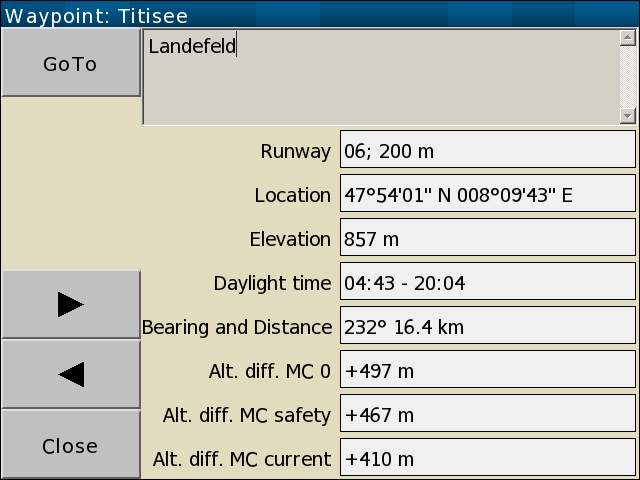
\includegraphics[angle=0,width=0.8\linewidth,keepaspectratio='true']{figures/dialog-waypointdetails0.png}
\end{center}

As mentioned above, the Waypoint info dialogue also shows three forms of altitude 
difference (additional
altitude required to reach the waypoint at the safety height) for
the corresponding waypoint:
\begin{description}
\item[Alt diff MC 0] Altitude difference at MC setting of 0
\item[Alt diff MC safety] Altitude difference at the abort/safety MacCready 
  setting (see \ref{sec:safety-factor})
\item[Alt diff MC current] Altitude difference at the current MacCready setting
\end{description}

From the main Waypoint Info screen, you can access the second page by using the 
\bmenuw{$>$} and \bmenuw{$<$} buttons in the bottom left corner of the page.
\subsection*{Task actions menu}  
This page contains a column of buttons allowing various actions to be performed:
\begin{description}
\item[\bmenuw{Replace in task}] replaces the active waypoint in the task with 
  the selected waypoint.
\item[\bmenuw{Insert in task}] inserts the selected waypoint before the active 
  waypoint in
  the task.
\item[\bmenuw{Append to task}] adds the selected waypoint to the end of the task.
\item[\bmenuw{Remove from task}] removes the selected waypoint from the task.  
  Note that this option is only visible if the selected waypoint is included in 
  the active task.
\item[\bmenuw{Set as new home}] sets the waypoint as the home airfield.
\item[\bmenuw{Pan to waypoint}] switches to pan mode and pans to that waypoint.
\end{description}

It is a good idea to set your home waypoint from the waypoint details
dialogue. This causes XCSoar to start up at the home location regardless
of whether a GPS fix is received.  If no home is set, then XCSoar
starts in the centre of the terrain map.

\subsection*{Airfield information}
This page may contain relevant text from the en-route supplement about
the airfield, including runways, radio frequencies, traffic patterns,
contacts.
\begin{center}
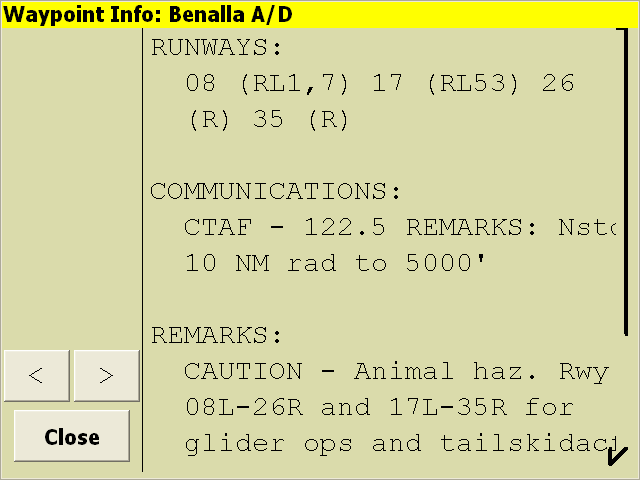
\includegraphics[angle=0,width=0.8\linewidth,keepaspectratio='true']{figures/dialog-waypointdetails1.png}
\end{center}

\subsection*{Waypoint details image}
This page shows a satellite image of the waypoint.

\begin{center}
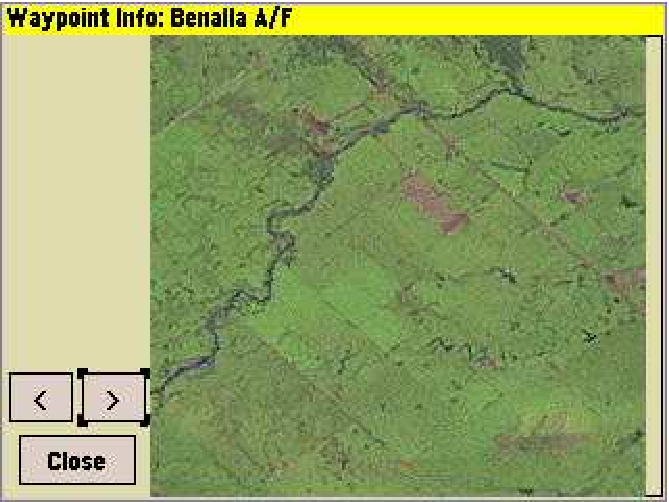
\includegraphics[angle=0,width=0.8\linewidth,keepaspectratio='true']{figures/dialog-waypointdetails2.pdf}
\end{center}
How to set up the detailed waypoint information read section \ref{sec:airfield-details}

\section{Waypoint selector dialogue}\label{sec:waypoint-selector-dialog}

The waypoint selector is a dialogue that allows waypoints to be easily selected
from a potentially large database. \gesturespec{dr}

Invoking the selector brings up a filtering dialogue screen with a set of 
\menulabelr{\bmenug{Nav 1/2}\blink\bmenug{Waypoint List}}
optional filters on the left side of the page, and a list of waypoints on the
right, matching all of the filtering conditions set.
There are several filters available, which may be used together,
individually or not at all.
\begin{description}
\item[Name] Selects waypoints, starting with the string typed.
\item[Distance] Filters out waypoints farther than a specified distance from the 
  aircraft.
\item[Direction] Filters out waypoints that are not in a specified direction 
  from the aircraft. 
  An additional special direction ``HDG(0°)'' filters waypoints within 30
  degrees to either side of the heading of the glider.  This allows the pilot 
  to point the glider at a group of waypoints and quickly find them.
\item[Type] Filters out waypoints that are not of the specified type
(Landable point, Airport or Turnpoint) or that appear in the specified File~1 or
File~2 (primary or secondary waypoint file respectively).
\end{description}
When filtering by name and type, the list of matching waypoints is
sorted by name. When (in addition) filtering by distance or direction,
 the list of matching waypoints is sorted by distance.

\begin{center}
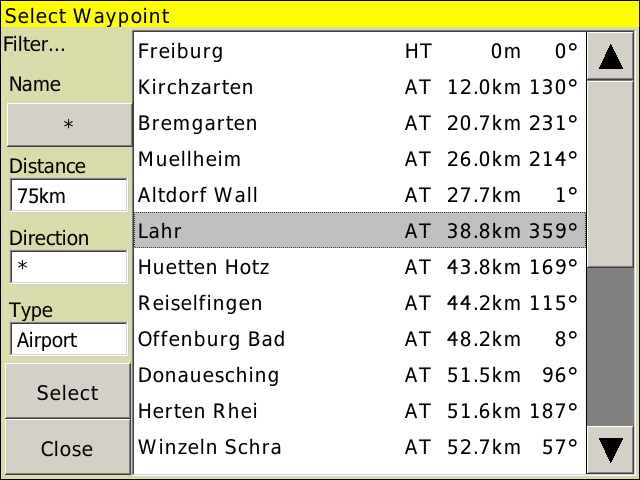
\includegraphics[angle=0,width=0.8\linewidth,keepaspectratio='true']{figures/dialog-waypointselect.png}
\end{center}

The list can be scrolled if there is more than one screen full of
matching waypoints.  To scroll through the list, simply drag with the finger, or
move to the bottom (or top) of the list with the cursor.   

Selecting an item will result in different behaviour
depending on what function opened the waypoint selector.  In typical
use it brings up the waypoint details dialogue for the selected
waypoint.

\section{Task manager}\label{sec:task-manager-dialog}
\begin{it}  The task manager has undergone significant redesign compared with 
earlier versions of XCSoar.\end{it}
\gesturespec{rd}

The task manager is used to edit, view, load, save to file, and declare cross
country tasks.
\menulabelr{\bmenug{Nav 1/2}\blink\bmenug{Task}}

The primary page is a calculator. It shows various calculations 
related to the active task, as described in detail below.  In addition, there 
are buttons for invoking dialogues \bmenuw{Turn Points}, \bmenuw{Manage}, 
and \bmenuw{Rules}, as well as a button to \bmenuw{Close} the task manager.

\subsection*{Task calculator dialog}\label{sec:task-calc-dial}
The task calculator dialogue allows the pilot to see the effect of
various changes to the task on final performance.
\menulabelr{\bmenuw{Calculator}}

In flight the Task Calculator might also be accessed from the Analysis pages. 
With pages Task, Climb, and Task Speed a button \bmenuw{Task Calc} comes up,
that directly changes to the Task Calculator screen.


\begin{center}
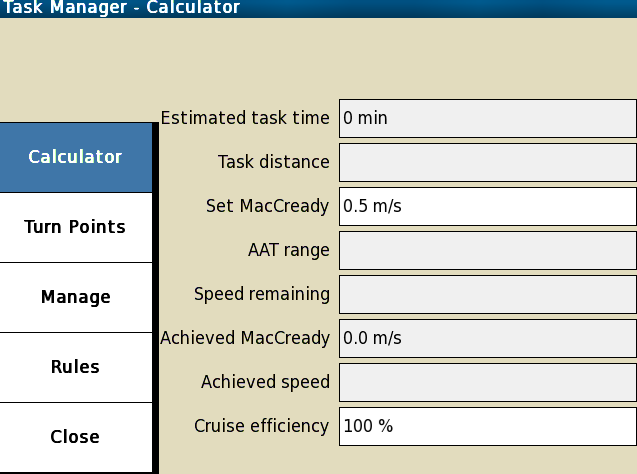
\includegraphics[angle=0,width=0.8\linewidth,keepaspectratio='true']{figures/dialog-taskcalculator.png}
\end{center}

\begin{description}
%\item[Assigned task time]  This field displays the assigned task time.
\item[Estimated task time]  This field displays the estimated total time 
  on task to complete the task at the provided MacCready setting.
\item[Task distance]  This field displays the task distance remaining.
\item[Set MacCready]  Allows the user to adjust the MacCready value and 
  see the effect it has on the estimated task time.
\item[AAT range]  Allows the user to adjust the targets within the remaining 
  AAT areas, to see the effect it has on estimated task time and task distance.
\item[Speed remaining]  This field displays the estimated speed for the
  remainder of the task at the provided MacCready setting.
\item[Achieved MacCready]  This field displays the achieved MacCready value.
\item[Achieved speed]  This field displays the achieved speed % at the achieved MacCready setting???
\item[Cruise efficiency]  100 indicates perfect MacCready performance, greater 
than 100 indicates better than MacCready performance is achieved through flying
in streets. Less than 100 is appropriate if you fly considerably off-track. This 
value estimates your cruise efficiency according to the current flight history 
with the set MC value. Calculation begins after task is started.
\end{description}
See Section~\ref{sec:task-speed-estim} for more details on task speed
and achieved MacCready calculations.

On closing the dialogue the entered MacCready value is used as the MacCready 
setting. If the \bmenuw{Cancel} button is pushed, the MacCready setting is 
unaffected.

The \bmenuw{Target} button, for AAT tasks, adjusts the range
(increases or decreases) so that the estimated task time exceeds the
assigned task time by less than five minutes.  The range is adjusted
target-wise. In typical use, all targets are set to ``auto'' that means the pilot
does not have to manually adjust the range to find the course for arrival at 
the assigned task time, thereby reducing pilot workload.

\subsection*{Turn Points}
This page displays an ordered list of the points in the current active task.
\menulabelr{\bmenuw{Turn Points}} 
If there are no waypoints in the active task, there 
will be only an option to ``Add Turnpoint.''  By highlighting (tapping) the
``Add Turnpoint'' function, then tapping in the highlighted region, the waypoint
selector is displayed, as described above.  Highlighting a waypoint from the 
list and then tapping on the highlighted region adds the waypoint to the task.

\subsection*{Manage}
This page allows for invoking all operations needed to create new or manage 
\menulabelr{\bmenuw{Manage}}already defined tasks.


\begin{itemize}
\item [\bmenuw{New Task}] Clears the current task and resets the task rules to 
  the default values.
\item [\bmenuw{Declare}] If an external logger is connected, this will allow 
  uploading the  active task to the logger and declaring it.
\item [\bmenuw{Browse}] Displays a list of all the saved tasks, allowing the 
  pilot to load a previously saved task.  Note that this option will overwrite 
  the current active task.
\item [\bmenuw{Save}] Saves the current active task.  Upon tapping the 
  \bmenuw{Save} button the pilot will be prompted to enter a file name for the 
  task to be saved.
\end{itemize}

\subsection*{Rules}
The values in the menu depend on the task type selected. Clicking any existing 
\menulabelr{\bmenuw{Rules}} value will bring up another menu allowing the pilot to select a 
different value for this rule.  Task types are discussed in more detail below.

Also, tapping on the \bmenuw{Rules} button again after it is highlighted allows 
toggling between a ``thumbnail'' view of the task map and a larger view of the task.

\section{Task types}
XCSoar currently defines three different task types: Racing, AAT, and FAI badges/records.

A brief description of the task types is included below, but this manual does 
not intend to rephrase FAI rules or contest task types. The reader is encouraged 
to become thoroughly familiar with each task type by referring to contest rules 
or FAI rules, which are available at \url{http://www.fai.org}. 


\subsection*{Racing}
(also known as an ``assigned task'').  The racing task involves flight
around each specified turnpoint in the specified order.  Selecting the racing task 
type allows the pilot to enter the following parameters.
  \begin{description}
  \item [Arm start manually] If set to ``On'', some extra buttons are presented 
  in order to let you \bmenug{Arm start} as well as \bmenug{Disarm start} in 
  menu \bmenug{Nav 1/2}, controlling  the detection of the start condition.
  \item [Start open time] This is the time when the start zone opens.
  \item [Start close time] This is the time when the start zone closes.
  \item [Start max.\ speed] This is the maximum speed allowed in the start observation
    zone.  This should be set to 0 if there is no limit.
  \item [Start max.\ height] This is the maximum height above the start height
    reference (AGL or MSL) at which a task can be started.  This  should be set to 
    0 for no limit.
  \item [Start height ref.] This specifies whether the maximum start height is 
    referenced to ground level of the start point (``AGL'') or Mean Sea Level (``MSL'')
  \item [Finish min.\ height] This is the minimum height based on the finish
    reference (AGL or MSL) at which a task can be finished.  This should be set to 
    0 for no limit.
  \item [Finish height ref.] This specifies whether the minimum finish height 
    is referenced to ground level of the finish point (``AGL'') or Mean Sea Level (``MSL'')
% \item [FAI start/finish rules] If enabled, this task type has no max.\ start height
%   or max.\ start speed.  Finish height reference is set to AGL and finish height
%   is 1000m below the start height \todonum[inline]{Is this description correct?}
  \end{description}
  
\subsection*{Assigned area task (AAT) and Modified area task (MAT)}
(also known as ``Turn Area Task,''or TAT).  This is a task through assigned
areas (restricted to cylinder or sector observation zones).  A minimum task time 
applies.  Rules options for this task type include:
  \begin{description}
  \item [AAT min.\ time]  This is the required minimum time for the task.  Refer
    to contest rules or consult an expert for penalties associated with finishing 
    prior to the minimum time.  The time in this option is given in minutes.
  \item [other rules] All other rules stay the same as in case of task type 
    ``racing''.
  \end{description}


\subsection*{FAI badges/records}
  \begin{description}
  \item [FAI start/finish rules] If set to ``On'', only start times might be set. 
  If set to ``Off'', all other racing task rules might be altered from the FAI standard.
  \end{description}

Once the appropriate task type has been selected and start and finish rules 
have been defined as described above, it is necessary to define the properties 
of each waypoint in the task.  

\section{Turn Points' task rules}\label{sec:task-rules}

The \bmenuw{Turn Points} dialogue brings up the list of waypoints in the task. 
\menulabelr{\bmenuw{Turn Points}} If no waypoint is already defined, this screen 
will show an empty list. With \bmenuw{(add Turnpoint)}, up and down arrows, and 
\bmenuw{Make Finish} an ordered list of waypoints is created. 
Waypoints can be start point, turnpoint, or finish point.
Highlighting any waypoint on the list and either tapping it again or 
touching the \bmenuw{Edit Point} button brings up the waypoint definition. 
Touching \bmenuw{Change type} will bring up a menu of the various task point 
types available.  Definitions of each point type are given below.

A variety of task rules may be used when specifying tasks, including
the common FAI triangles and Assigned Area Tasks (AAT).  Many aspects
of the rules can also be customised.

Starting and finishing lines are centred on their associated waypoint
and aligned perpendicular to the next and previous waypoints
respectively.

Sector turn-points are 90 degree segments aligned to the bisection of
the previous and next waypoints, as commonly used in FAI tasks.
There is also support for British BGA, and German DAeC sectors.

\subsection*{Start point types}
The conditions to be met for a valid start depend on the type of start:
\begin{description}
\item[Start Cylinder] When the glider leaves the cylinder area.
\item[Start Line] When the glider crosses the start line.
\end{description}

\subsection*{Turnpoint types}
The conditions to be met for a valid turnpoint pass depend on its
 type:
\begin{description}
\item[FAI Sector] When the glider has entered the observation zone (OZ), defined 
by a segment and radial distance from the waypoint.  The segment is
defined by a 90 degree arc centred about the bisector of inbound and
outbound legs, with a distance of 20 km.
\item[Keyhole Sector (DAeC 0.5/10 sector)] When the glider has entered the
observation zone, defined by a segment and radial distance from the waypoint.  The segment is
defined by a 90 degree arc centred about the bisector of inbound and
outbound legs, with a distance of 10 km.  The observation zone also includes
a cylinder of 500 m.
\item[Turnpoint Cylinder]  When the glider has entered the observation zone
defined by a radial distance from the waypoint.
\item[BGA Fixed Course Sector]  When the glider has entered the
observation zone defined by a segment and radial distance from the
waypoint. The segment is defined by a 90 degree arc centred about the
bisector of inbound and outbound legs, with a distance of 20 km.
The observation zone also includes a cylinder of 500 m (British rules).
\item[BGA Enhanced Option Fixed Course Sector]  When the glider has entered the
observation zone defined by a segment and radial distance from the
waypoint. The segment is defined by a 180 degree arc centred about the
bisector of inbound and outbound legs, with a distance of 10 km.
The observation zone also includes a cylinder of 500 m (British rules).
\item[Area Zylinder (AAT)]  and
\item[Area Sector (AAT)]  When the glider has entered the observation zone
defined by the radial distance from the waypoint, and segment for sector areas.
\end{description}

\subsection*{Finish point types}
Task completion depends on the finish type:
\begin{description}
\item[Finish Cylinder] When the glider enters the cylinder area.
\item[Finish Line] When the glider crosses the finish line.
\end{description}

Automatic advancement is triggered whenever a condition is met. To start an AAT,
mixed task, or Racing task the start has to be armed before. 

\tip Competition rules may be defined in a profile file for
distribution to a group of pilots or task-setters, so all competitors
are playing by the same rules!

Additional task rules for valid starts and finishes may also be
specified.  Starts may have a defined maximum altitude above ground,
and a maximum speed.  Finishes may have a minimum altitude above
ground.  These parameters are defined in the page ``Default Task Rules'' in
the configuration \config{taskrules} settings.

For non-AAT tasks, an option is available to set the minimum finish
altitude according to the FAI rule, whereby the minimum finish
altitude is above 1000 meters below the start altitude.


%Need to add a section describing how to start the task%


\section{Advancing and restarting tasks}\label{sec:advanc-rest-tasks}
At all times one waypoint in the task is designated as the active
waypoint.  The active waypoint is used for calculation and display of
navigation information, that is, the pilot is directed to fly towards
the active waypoint (also referred to as the ``next waypoint'' in the
description of InfoBoxes as in Chapter~\ref{cha:infobox}).

During flight a continuous display of the bearing to the next waypoint is shown.

The altitude required to complete the task is calculated for the route starting
from the glider's actual position going through the task's turnpoints to the 
final waypoint.

Changing the active waypoint is performed automatically, or may be performed manually.
The start point of racing tasks, and AAT task points, are special cases that require
the task point to be ``armed'' before the system will automatically advance to the next
task point once that point is reached.  All other task points will automatically
advance to the next point as soon as the last point was reached.

For non-racing tasks, no user interaction is required to
advance through the task --- the system will automatically advance as
each task point is achieved.  The user may still manually advance or retreat the active
task point by selecting the menu items \bmenug{Nav}\blink\bmenug{Previous turnpoint} and
\bmenug{Nav}\blink\bmenug{Next turnpoint} respectively.

The menu items \bmenug{Previous turnpoint} and
\bmenug{Next turnpoint} show dynamic labels that
indicate the action that will be performed upon selecting the item.

For task points requiring arming, \bmenug{Next Turnpoint} becomes 
\bmenug{Arm turn} if the turn is not armed; if it is armed, then it becomes 
\bmenug{Next Turnpoint} allowing for manual advance. 
\bmenug{Previous Turnpoint} changes to \bmenug{Disarm turn} if the turn is armed 
and vice versa. Similarly, for racing tasks these menu items update for arming 
start points. If the Next Turnpoint is the \bmenug{Finish Turnpoint}, the menu 
label changes accordingly.

Status messages are given for task points requiring arming, when
inside the observation sector, as reminders to arm the turn when the
pilot is ready to advance to the next waypoint. For starting, a
warning is given that the glider is in the start cylinder or behind
the start line, as a reminder to ``arm'' if necessary.

For PC and Pocket PC with touchscreen versions only, the user may
manually cycle through the waypoints by highlighting the waypoint
{\InfoBox} and by pushing the up or down cursor key.

See Section~\ref{sec:task-rules} for details on observation rules.

If a user has cycled through the waypoint manually, this does not mean
that the glider has successfully passed the waypoint!  However, this
facility is useful to force a task restart or to skip a waypoint when
flying a casual cross-country task.

\tip Tasks can be restarted simply by manually cycling back through the
waypoints to the start.

In all modes, if the glider re-enters the start zone or crosses the
start of the previous start, the task will be automatically restarted. 

When selecting \bmenug{Previous turnpoint}, the trigger that detects
auto-advance for that waypoint is cleared; meaning that the task
manager expects the aircraft to fly to that observation zone (OZ)
again before continuing the task. The pilot may still select \bmenug{Next
turnpoint} to advance to the next task waypoint.

A system beep and message is given on task/waypoint advance.  The
messages are given when the system advances the task waypoint
automatically or, in manually arm mode, when the system is armed and the
aircraft is in sector:
\begin{description}
\item[Task start]  appears when the aircraft has crossed the start line or
 exited the start sector. This can be repeated any time.
\item[Next turnpoint]  appears when the aircraft has entered the observation
 sector for turnpoints. Turns with variable target advance as soon as
 \button{Arm Turn} is pushed.  For the manual arm mode, if the
 aircraft has already entered the observation sector and left, pushing arm will
 cause the task manager to expect, that the turn is intended to approach
 another time.
\item[Task finish]  appears when the aircraft has crossed the finish line
 or entered the finish cylinder.  This occurs in both advance modes. 
\end{description}


\section{Alternate starts}\label{sec:alternate-starts}

%Alternate start points are skipped for XCsoar 6.0, but
%will potentially brought back in a next release. 

%\todonum[inline]{Alternate start points are skipped for XCsoar 6.0, but
%will potentially brought back in a next release. This section can thus be
%treated as obsolete. }

The task system allows alternate start sectors to be defined:

\blink\bmenuw{Turn Points} select start point, \menulabelr{\bmenug{Nav 1/2}\blink
\bmenug{Task}}\bmenuw{Edit Point}\blink\bmenuw{Enable Alternate Starts}

On the start point edit page of the Task Manager turn on the \bmenuw{Enable 
Alternate Starts} property. Another screen is brought up for defining an 
alternate start point. In case, alternate start points have been defined before, label \bmenuw{Enable Alternate Starts} changes to \bmenuw{Edit Alternates}. After selecting ``Add Alternate Start'' and touching 
\bmenuw{Relocate} the ``Select Waypoint'' filtering dialogue is invoked.

Having set up several alternate start points, the ``next waypoint'' scheme again will be extended. Before detection of a valid start and having armed start manually, the menu buttons stepping through all the waypoints will show label \bmenug{Next Start}.

Summarizing, all dynamic menu labels in menu \bmenug{Nav 1/2} show commands to be 
executed for selecting waypoints and conditions either consecutively or in reverse 
order. 

%\begin{center}
%\includegraphics[angle=0,width=0.8\linewidth,keepaspectratio='true']{figures/%dialog-startpoint2.png}
%\end{center}
  
%  To edit the start points, move the cursor to an item in the list on
%  the right side of the dialogue, and press enter.  This opens the
%  waypoint selector dialogue, to allow selection of the waypoint.  This
%  process can be repeated several times for several alternate start
%  waypoints.  Press the `clear' button to clear all alternate start
%  points.

%  Each start sector is fixed to the same type (line/cylinder) and size
%  (start radius) defined in the task waypoint page.

%  Note that the task start point should be included in the alternate
%  start location list. 

%\begin{center}
%\includegraphics[angle=0,width=0.8\linewidth,keepaspectratio='true']{figures/%dialog-startpoint3.png}
%\end{center}

%\begin{center}
%\includegraphics[angle=0,width=0.8\linewidth,keepaspectratio='true']{figures/%dialog-startpoint4.png}
%\end{center}

%  In flight, any time you cross a start line (or exit a start
%  cylinder), this will start the task at that particular alternate
%  start.  Task statistics are recalculated for the start sector you
%  last flew through.  All alternate start sectors are shown on the
%  map.  You can re-start simply by flying through the start sector
%  again or another start sector.  This automatic re-start will only
%  happen if the active waypoint is the first turnpoint after the
%  start, or the start itself.

%  When the waypoint advance mode is `Arm' or `Arm Start', then a start
%  is only recognised by XCSoar if the advance trigger is armed.

%  If desired, alternate start points may be selected as the active
%  waypoint by selecting the previous waypoint.  Continuing to select
%  the previous waypoint will cycle through all alternate start points.

\section{Abort/resume the task and Alternates}

If atmospheric conditions change for the worse, you may make the
judgement that it will be impossible to complete the task.  In this
situation, XCSoar can be instructed to ``abort'' the task, and it will
then help you reach a safe landing site. An ordered task can be aborted in 
different ways. Either it is done by selecting a waypoint and execute the goto 
command or by invoking the abort mode. In either case, the ordered task might be resumed.

\subsection*{Task Abort}\label{sec:taskabort}
Invoking the abort mode forces XCSoar to enter a special case of the final glide mode. \menulabelr{\bmenug{Nav 2/2}\blink\bmenug{Task Abort}} For a discussion on 
flight modes refer to section \ref{sec:flightmodes}. In this flight mode
the configuration option `reach polar' determines whether
waypoint arrival heights in abort mode uses the MacCready value prior
to aborting the task, or if the safety MacCready value is used. \config{reachpolar}
Default is to use the safety MacCready value.  When switching to
abort mode, the MacCready setting is set to the safety value 
if it is lower than the current setting.

With invoking abort mode the cross-country task is disabled. On the map radials 
are drawn pointing to the nearest landables to instantly 
support the pilot's decision. As is during the whole flight, the group of nearby 
landables is maintained permanently. Radials and nearest landables may change 
dynamically when in abort mode, so that at any time several landing options are 
presented and any of these may be selected as the active waypoint. Even if no 
landable is in reach, the radials are drawn.
\sketch{figures/abort-low.png} 
If conditions improve, the task can be resumed by selecting the same
menu button that aborted the task, now denoting \bmenug{Resume Task}. The active 
waypoint, prior to aborting the task, is then restored along with all the other 
task details.

\subsection*{Alternates} \label{sec:alternates}
Alternates are maintained throughout the flight, reflecting good airmenship by 
always keeping an eye on possible alternates.\menulabelr{\bmenug{Nav 1/2}\blink
\bmenug{Alternates}} Six landing 
options are maintained. They are filtered by the configured ``alternates mode'' 
criteria (Simple, Task, or Home). \config{alternatesmode} 
Choosing Task or Home puts some bias on the presentation of alternates to the 
heading, you were taking whilst still task oriented.

As is with every waypoint list, additional information might be called by tapping \bmenuw{Details} before deciding which final to go. Select a waypoint from the list and push \bmenuw{Goto}.
\sketch{figures/alternates_list.png}

Although the items on the alternate list obey different rules they interact 
in the same way 
with the current task. Choosing a target from the alternates list aborts the task; 
once the conditions get better the resuming of the task is doable by the already 
mentioned button.


\section{Task status}\label{sec:task-status}

The status dialogue gives a summary of important task information. 
\gesturespec{ldrdl} It can be useful to give a
good overview of the task status while freeing up InfoBoxes for other
purposes.  The status dialogue can be referred to in order to confirm
that a valid start was detected, as well as the progress against the
task.
\menulabelr{\bmenug{Info 2}\blink\bmenug{Status}}
The status dialogue can be invoked by menu or gesture left down right down left, denoting an S. The status tabs `Task' and `Rules' are of interest.

The task tab shows the AAT times, distances achieved and remaining and the 
task speeds. The rules tab shows the validity of start/finish according 
to the task rules.
\begin{center}
\begin{tabular}{c c}
Task & Rules \\
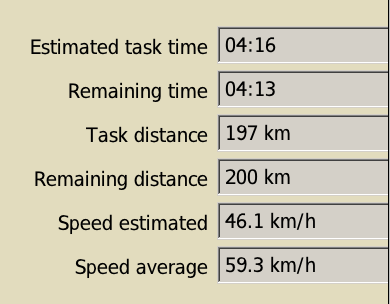
\includegraphics[angle=0,width=0.4\linewidth,keepaspectratio='true']{figures/status-task.png} &
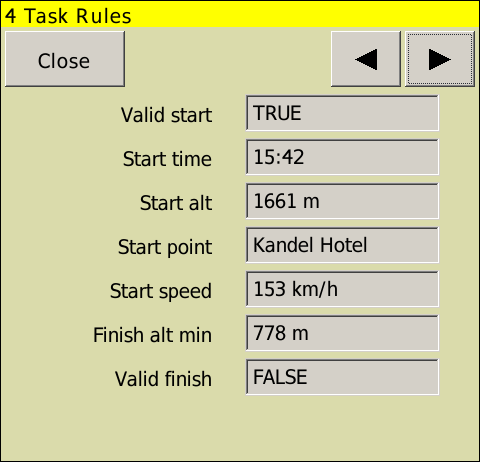
\includegraphics[angle=0,width=0.4\linewidth,keepaspectratio='true']{figures/status-rules.png} \\
\end{tabular}
\end{center}

\section{Assigned Area Tasks}\label{sec:aat-tasks}

\subsection*{AAT targets}

A {\em target} is a point within an AAT area that the pilot intends to
fly to.  These targets can be moved within the AAT areas so the pilot
can adjust the effective distance of the task.  Targets may be set on
the ground, during task planning, and modified during flight.

When flying an AAT task, the navigation system directs the glider to
the target, and statistics like distance to waypoint are also relative
to the target rather than the waypoint of the AAT area itself.

Automatic task waypoint advancement does not trigger when entering an
AAT area solely. The pilot has to arm the turn manually to advance to the next
turn. When arming the AAT turn while flying through the OZ also the task
optimiser is triggered to capture the realized AAT target and bring the target
optimisation for the rest of the task up to date. See Section~\ref{sec:advanc-rest-tasks} 
for details.

\subsection*{Manually moving targets}

In order to make the specification of targets more straightforward,
their location is defined by a range parameter that determines how
far from the minimum to maximum possible distance the target is.  This
is expressed as a percentage.  For example, with range set to 100\%,
the target is located to give the maximum overall task distance.  With
range set to~$-100$\%, the target is located to give the minimum overall
task distance.  

Zero range yields a nominal task distance: for sectors the target is
half way along the bisector radial; for cylinders the target is in the
center of the cylinder.

The task calculator dialogue (see Section~\ref{sec:task-calc-dial}), shows the
average percentage over all turns in the AAT Range field.
The targets can be individually modified from the target dialogue of the task
calculator.


\subsection*{AAT targets and the Task Calculator}

The typical use of targets in flying AAT is as follows:
\begin{itemize}
\item Set the expected MacCready, bugs/ballast and wind settings
  for the flight using the flight settings and wind settings dialogues.
\item Define the task as normal from the task editor.
\item Based on the pilot's judgement of how good the weather is,
  and whether some areas are likely to be more or less difficult than
  others, targets may be set individually for each turn-point in the
  target view.  The ETE field in the target view compared to
  the assigned minimum time is shown as Delta T to check if the planned 
  task is efficient and long enough.
\item During flight, if situations change, such as changed MacCready setting
  or wind, the task calculator can be brought up to show the estimated
  task time, again allowing comparison to the assigned minimum time.
\item If the pilot decides to extend or shorten the flight, all the remaining
  targets can be modified from the task calculator. 
\end{itemize}

The task calculator therefore allows the pilot to make (and help to
answer) `what if?' questions, for example:
\begin{itemize}
\item What will happen if the conditions improve?  The MacCready setting can be 
increased and the pilot can see if there is sufficient adjustment to targets in 
order to be able to extend the planned task.
\item What will happen if the conditions deteriorate?  The MacCready setting can 
be decreased and the pilot can see how much the task can be shortened and still 
finish the task later than the assigned minimum time.
\item What will happen if I leave the AAT area now?  By pressing \button{Arm
turn} the take over of the current position into the optimization can
be forced. The repositioning of subsequent turns can be reviewed in the task calculation
dialogue.
\end{itemize}

\subsection*{Target projection}

XCSoar continually analyses the path of the glider through AAT sectors
to find the points in previous AAT sectors through which the achieved
scoreable distance will be greatest.  Internally, the program moves
the targets for previous AAT sectors, which are then the optimal
targets.

In certain conditions, targets for the current AAT sector may be moved
automatically:
\begin{itemize}
\item When inside an AAT sector, the target in that sector is moved to
to a line projecting from the previous sector's target through the
aircraft, at the same distance from the previous sector's target to
the target prior to entering the sector.  The effect of this is to
allow pilots to choose to enter an AAT sector in a different direction
or offset from the direct line from the previous target to the current
target.

\item While the aircraft is in the AAT sector and the distance from the
previous target to the aircraft is greater than the distance from the
previous target to the current target, the target is moved further
along the projected line from the previous target to the aircraft,
just beyond the aircraft.  Hence, the black track line will not be
visible but the blue optimal track arrow will point along this
projected direction.
\end{itemize}

A worked example is provided in the following figures to illustrate
how targets move during a flight and to show how XCSoar determines the
maximum scored path.

\begin{maxipage}
\begin{center}
\begin{longtable}{|c|c|}
\toprule
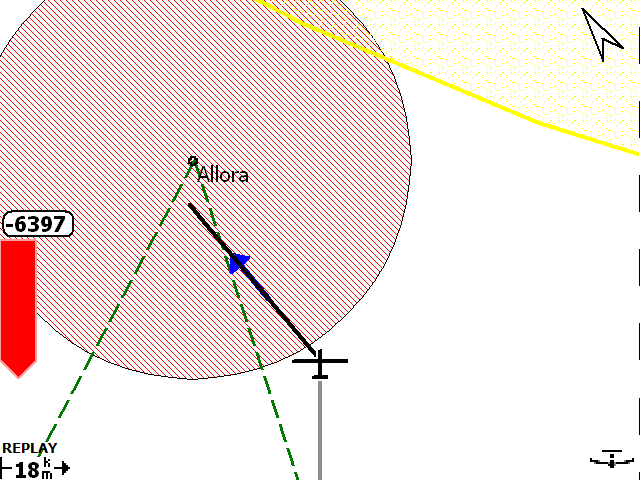
\includegraphics[angle=0,width=0.45\linewidth,keepaspectratio='true']{figures/faat01.png} & 
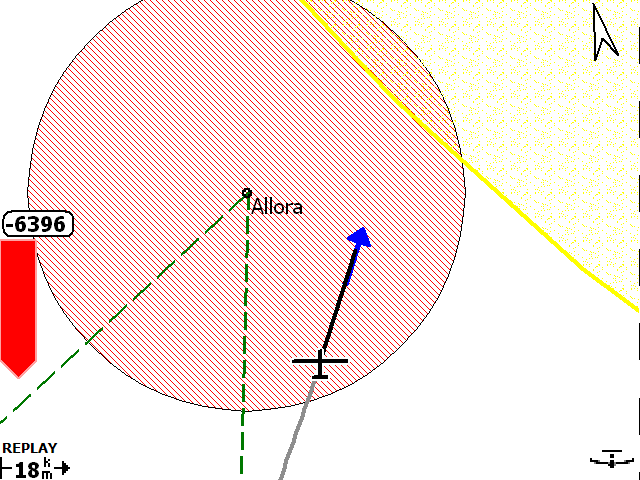
\includegraphics[angle=0,width=0.45\linewidth,keepaspectratio='true']{figures/faat02.png} \\
{\em Outside sector} & {\em Inside sector} \\
Target (-20\%) is on bisector & Target moved along track line \\

\midrule
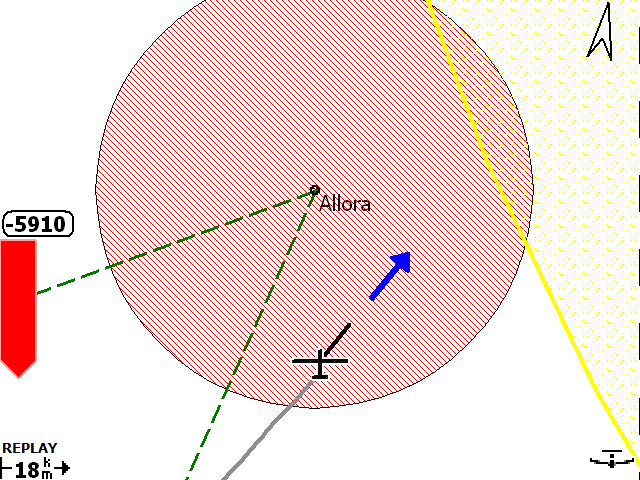
\includegraphics[angle=0,width=0.45\linewidth,keepaspectratio='true']{figures/faat03.png} & 
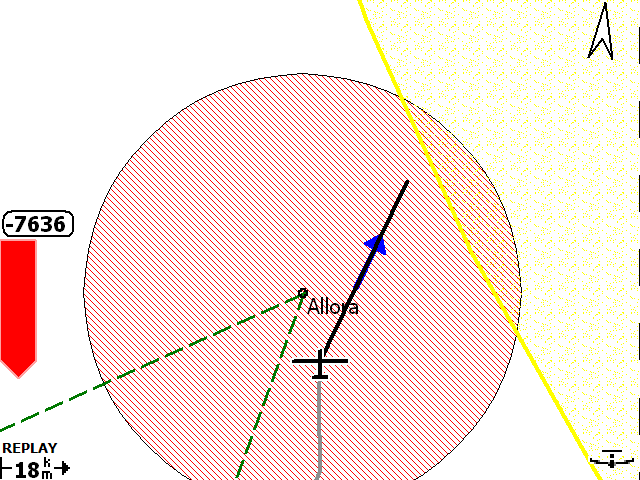
\includegraphics[angle=0,width=0.45\linewidth,keepaspectratio='true']{figures/faat04.png} \\
{\em User decreased range} & {\em User increased range} \\
Target (-80\%) moved along track line & Target (80\%) moved along track \\

\midrule
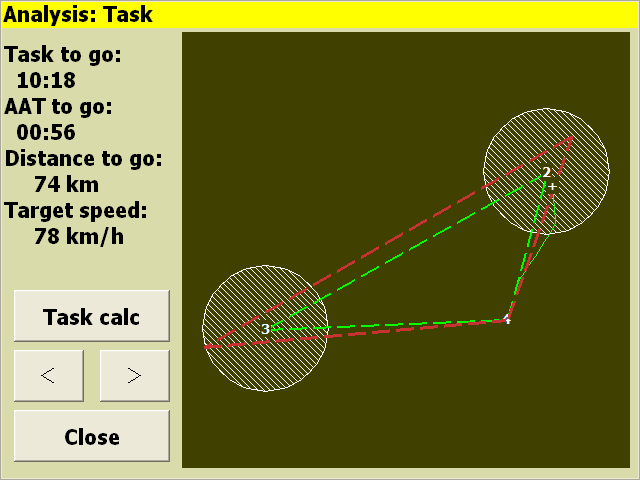
\includegraphics[angle=0,width=0.45\linewidth,keepaspectratio='true']{figures/faat05.png} & 
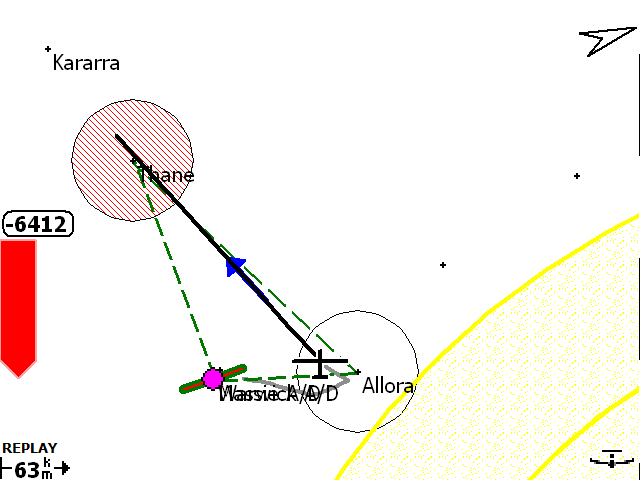
\includegraphics[angle=0,width=0.45\linewidth,keepaspectratio='true']{figures/faat06.png} \\
{\em Analysis (task page)} & {\em Next waypoint} \\
Path around active target  & ``Arm Turn'' pressed \\
\bottomrule
\end{longtable}
\end{center}
\end{maxipage}

\begin{maxipage}
\begin{center}
\begin{longtable}{|c|c|}
\toprule
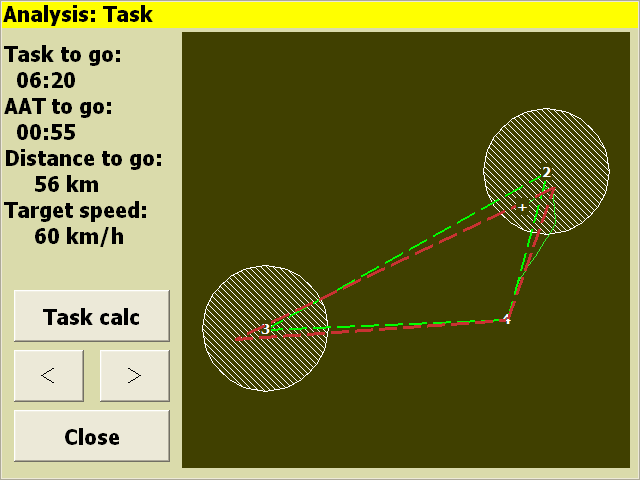
\includegraphics[angle=0,width=0.45\linewidth,keepaspectratio='true']{figures/faat07.png} & 
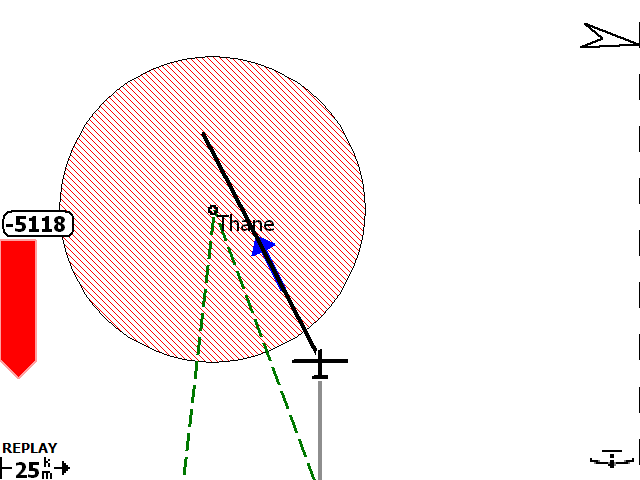
\includegraphics[angle=0,width=0.45\linewidth,keepaspectratio='true']{figures/faat08.png} \\
{\em Analysis (task page)} & {\em Approaching next area} \\
Best scored target found & Target (60\%) is on bisector \\

\midrule
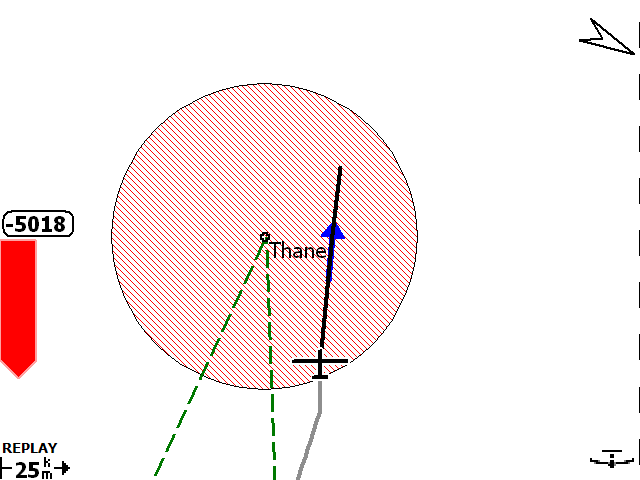
\includegraphics[angle=0,width=0.45\linewidth,keepaspectratio='true']{figures/faat09.png} & 
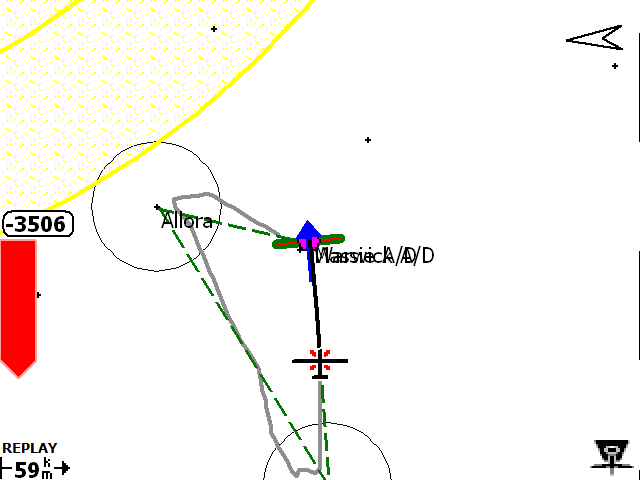
\includegraphics[angle=0,width=0.45\linewidth,keepaspectratio='true']{figures/faat11.png} \\
{\em Inside sector} & {\em Next waypoint} \\
Target (60\%) moved along track line & ``Arm Turn'' pressed \\

\midrule
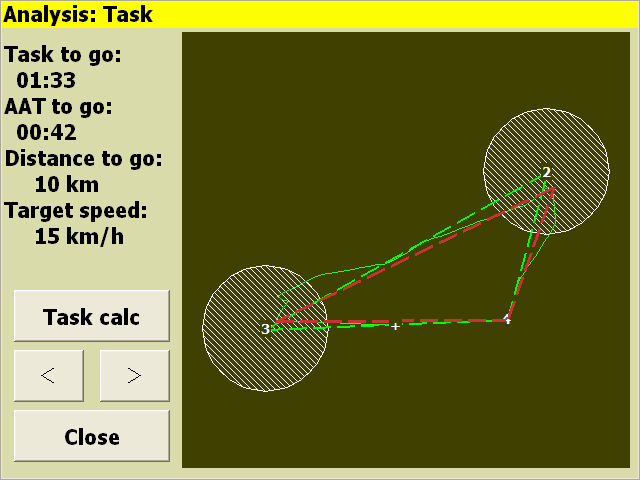
\includegraphics[angle=0,width=0.45\linewidth,keepaspectratio='true']{figures/faat12.png} &  \\
{\em Analysis (task page)} &  \\
Best scored targets found &  \\

\bottomrule
\end{longtable}
\end{center}
\end{maxipage}

\section{OnLine Contest}

The analysis dialogue contains a page ``OnLine Contest'' which can be
used to show the optimal path and estimated score.  The configuration settings \config{taskrules} 
(task rules page) allows the selection of which set of rules to be used for the
OLC optimisation.

The optimization is done continuously in the background and can be retrieved at
any time. The analysis page shows a graphical overview of the optimisation
result besides distance and score. A InfoBox is available which gives the
instant OLC distance and score as well.

\begin{center}
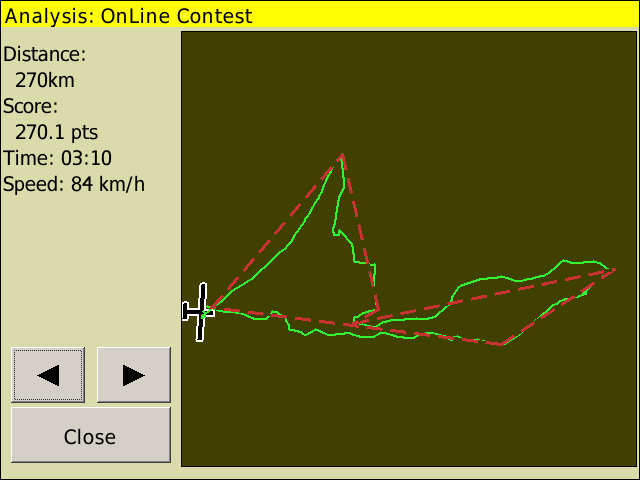
\includegraphics[angle=0,width=0.8\linewidth,keepaspectratio='true']{figures/shot-olc.png}
\end{center}

When flying OLC, either AAT or non-AAT tasks may still be used to
manage the flight navigation.  During flight, the computer will optimise the
current flight with respect to the selected OLC rules.  

In the OLC analysis page, the aircraft track is shown as a thin green line, the optimal 
path is shown as a thick red line.

The score and computed optimal distance is approximate.

When the aircraft has landed, the displayed result gets not updated anymore.


\section{Logger}\label{sec:logger}

A flight logger conforming to the IGC file specification can be used
to record flights.  

Several flight loggers are accessible via XCSoar:
\begin{itemize}
\item A software-based logger.  All versions of XCSoar have this
  functionality.  The logger conforms to the IGC standard but is not
  certified.
\item XCSoar can also send declarations to some external logger devices. 
  For this to work, the device must be specified in the `Devices' 
  section of the configuration \config{comdevices} settings.
\item  For some of the numerous logger devices XCSoar can download IGC files. 
  This is convenient especially for logger devices which are not that easily
  removable from the glider.
\end{itemize}

\subsection*{Setup}
For a complete matrix of the supported logger features see Section~\ref{sec:supported-varios}.
The configuration is described in detail in Section~\ref{conf:logger}.  Details
to the log files can be found in Section~\ref{sec:logfiles}.

\subsection*{Logger activation}
The logger can be turned on and off automatically or manually.  For para-glider 
XCSoar provides the option to only start the logger automatically. Thus a very 
slow and close to the terrain flight won't automatically stop logging the flight. 
If you choose the auto start only logger you have to stop the logger manually.
To turn the logger on (or off) manually, select from the menu:
\sketch{figures/logger-startdeclare.png}
\begin{quote}
\bmenug{Config 3}\blink\bmenut{Logger}{Start}
\end{quote}

When the internal software logger is active, a small `green status led' in the
lower right corner of the map area flashes once per second.

By default, XCSoar is set up to automatically start and stop the
internal software flight logger when it detects the aircraft is flying
and when it has landed, respectively.  Only when the logger is
manually started does it ask if the flight is to be declared; when
automatically starting it automatically declares the current task.
In simulation mode the logger does not get activated automatically.

If a task has been declared, then subsequent attempts at modifying the
task result in a warning message asking to confirm whether the action
is to be taken and invalidate the declaration.  This is intended to
make it harder to accidentally modify the task resulting in a failed
declared task.

The XCSoar software logger, when started, checks for 500kB of free
space on the file storage.  If there is insufficient space, it will
automatically delete IGC files, oldest first, in order to free up
500kB.  It does not ask the user for confirmation before performing
this operation. \warning

The internal software logger buffers data so that when it starts
(automatically or manually) up to 60 seconds of data prior to starting
is recorded.  This means that the software logger now adequately
captures the full take-off.

\subsection*{Logger replay}\label{sec:logger-replay}
Flight logs in the IGC format generated by XCSoar or other loggers can
be replayed.  The logger replay dialogue can be accessed via the
menu:
\begin{quote}
\bmenug{Config 2}\blink\bmenug{Replay}
\end{quote}
\sketch{figures/loggerreplay.png}

During replay, the word `REPLAY' appears at the lower left corner of
the screen.  During replay, the program behaves as if real GPS updates
are being received by a GPS.  The logger replay dialogue does not need
to be open during replay.

To start a log replay, first select the file to load, and then select the
\button{Start} button.  The replay can be performed in accelerated time
by changing the time scale from 1x to a higher number, and paused by
setting the time scale to zero.  High time scales can result in degraded
performance of the wind estimation and other statistics/analysis routines.

Stop the log using the \button{Stop}.
Once a log is started, further presses of the \button{Start} has the
effect of restarting the replay.

\tip It is recommended to reset the device before flight, after a log
file has been replayed, in order to ensure that XCSoar's internal
statistics are properly reset.

When operating XCSoar in FLY mode, the replay is disabled (stopped) if
the real GPS receiver detects that the aircraft is moving.

The logger replay works best with high sampling rate log files;
a 6 second interval or less works fine.

\subsection*{Error analysis logger}\label{sec:raw-logger}
For the pure reason of tracking down error prone behaviour of XCSoar 
there is a `Raw Logger'. In case you are able to reproduce an error you can 
activate the raw log file creation by:
\begin{quote}
\bmenug{Config 3}\blink\bmenug{Raw Logger}
\end{quote}
Developers will appreciate very much any detailed error description including a log file like this. It really facilitates the root cause analysis and saves time to fix an error.

\section{Flight analysis} \label{sec:analysis-climb}

The analysis dialogue is very useful in planning and conducting
cross-country flights.  It is accessed via the menu:  \gesture{Up - Right - Down}
\begin{quote}
\bmenug{Info 1}\blink\bmenug{Analysis}
\end{quote}

Several pages are of interest:
\begin{description}
\item[Barograph]  Shows a graph of the history of the altitude of the glider.
  Statistics are used to estimate the thermal working band (average
  base and ceiling of climbs) and to estimate how the ceiling is
  changing over time.  The base and ceiling lines are drawn on the
  barograph.

  The `Settings' button opens the flight settings dialogue
  (e.g.\ to adjust the QNH)

\begin{center}
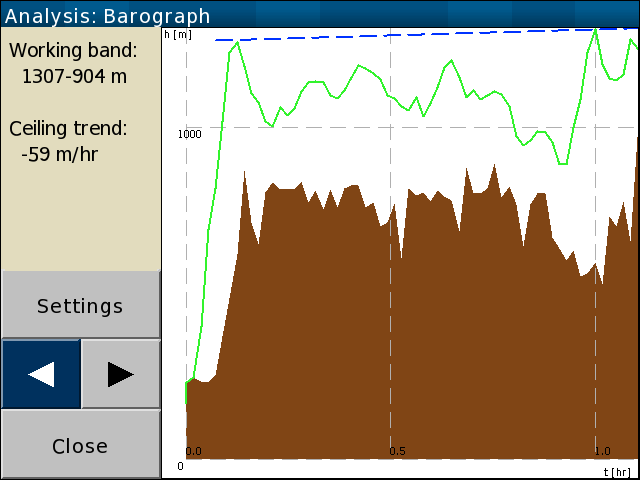
\includegraphics[angle=0,width=0.8\linewidth,keepaspectratio='true']{figures/analysis-barograph.png}
\end{center}

\item[Climb history]
  Shows a bar chart of the average climb rate achieved during each
  climb.  Statistics are used to estimate the overall average climb
  rate, and to estimate how this average is changing over time.  The
  current MacCready setting is drawn on the bar chart as a thick red
  dashed line, and the climb rate trend is drawn on the chart as a
  blue line.

  The ``Task Calc'' button opens the task calculator,
  (e.g.\ to adjust the MC value)

\begin{center}
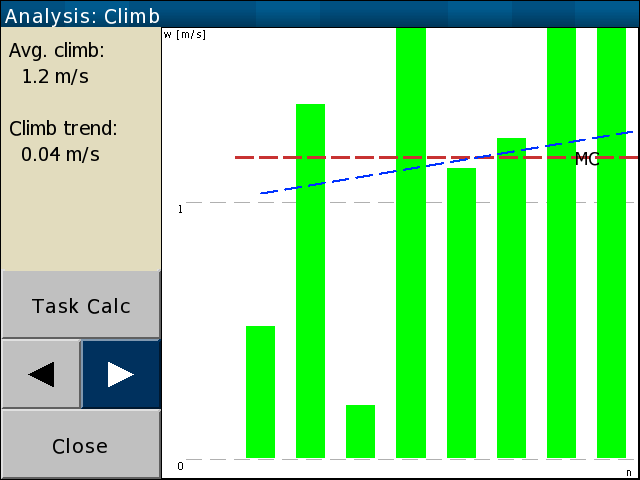
\includegraphics[angle=0,width=0.8\linewidth,keepaspectratio='true']{figures/analysis-climb.png}
\end{center}

\item[Task]
  This page shows an overview of the entire task.  The main task line
  is drawn in thick dashed green, AAT areas are shaded.  For AAT
  tasks, the path from the aircraft around the remaining targets within AAT
  areas is shown in red.  The aircraft track is shown as a thin green line.

  The `Task Calc' button opens the task calculator,
  (e.g.\ to adjust the AAT task range or MC value)

\begin{center}
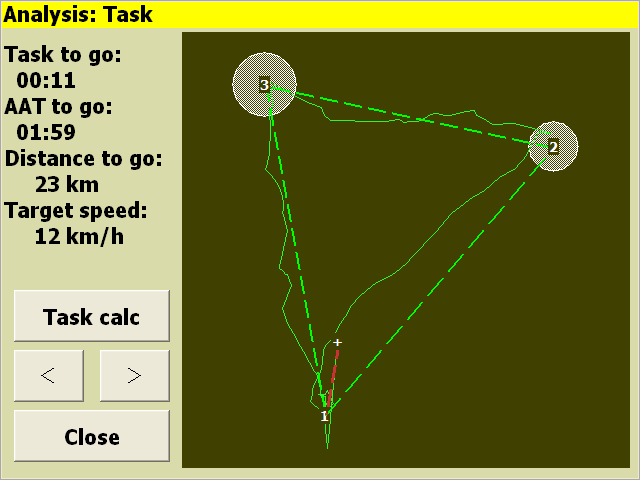
\includegraphics[angle=0,width=0.8\linewidth,keepaspectratio='true']{figures/analysis-task.png}
\end{center}

\end{description}

\section{Sunlight and time}

A sun ephemeris computes the time of sunrise and sunset, which is displayed in the
Aircraft Status dialogue (see Section~\ref{sec:time-status}).  Note that
local terrain and atmospheric conditions may result in poor visibility
before the displayed sunset time.

For PDA systems, the clock is adjusted for daylight saving time according
to the settings in the operating system.

If the expected arrival time at the final waypoint in the task is past
sunset, a status message warning is issued.
